\documentclass[12pt, letterpaper]{article}
\usepackage[T1]{fontenc}
\usepackage[utf8]{inputenc}
\usepackage{graphicx}
\usepackage{caption}
\usepackage{subcaption}
\usepackage{geometry}
\usepackage{float}
\usepackage{amsmath}
\usepackage{fancyhdr}
\usepackage{pdfpages}

% Page Geometry
\geometry{margin=1in}
\setlength{\headheight}{14.49998pt}
\addtolength{\topmargin}{-2.49998pt}

\graphicspath{{./Pictures/}}
\pdfcompresslevel=9
\pdfobjcompresslevel=3
\pdfminorversion=5

% Header/Footer Setup
\pagestyle{fancy}
\lhead{EEE3307: Lab 5 Report}
\rhead{Yousef Awad}
\cfoot{\thepage}

\title{
    \vspace{1in}
    \textbf{\huge EEE3307 Electronics I} \\[0.5em]
    \textbf{\Large Experiment \#5: Transistor Small-Signal Amplifiers}
    \vspace{1.5in}
}
\author{
    \textbf{Name:} Yousef Alaa Awad \\
    \textbf{Partners:} Egor Shevchenko and Abram Tadros
}
\date{Lab Session: April 9, 2026}

\begin{document}

\maketitle
\newpage

%----------------------------------------------------------------------------------------
%	1. INTRODUCTION
%----------------------------------------------------------------------------------------
\section{Introduction}
The objective of this experiment was to study the performance and characteristics of small-signal transistor amplifiers in two primary configurations: Common-Emitter (CE) and Common-Collector (also known as Emitter Follower). The experiment focused on measuring key parameters such as voltage gain ($Av_s$ and $Av_i$), input resistance ($R_{in}$), and output resistance ($R_{out}$). By comparing these two topologies, we can evaluate their relative advantages, such as the high voltage gain of the CE amplifier versus the unity gain but high input/low output resistance of the Emitter Follower.

%----------------------------------------------------------------------------------------
%	2. EXPERIMENTAL PROCEDURE
%----------------------------------------------------------------------------------------
\section{Experimental Procedure}
The experiment followed the procedures outlined in the EEE3307 Lab Manual for Experiment \#5:

\subsection{Common Emitter Amplifier}
\begin{enumerate}
    \item \textbf{Circuit Assembly:} A CE amplifier was built using $V_{CC}=12V$, $R_C=6.2k\Omega$, $R_E=1.8k\Omega$, $R_L=2.2k\Omega$, and $R_S=1.8k\Omega$. The bias resistors ($R_1 \approx 121k\Omega, R_2 \approx 35k\Omega$) were chosen to target $I_{CQ} \approx 1mA$.
    \item \textbf{Gain Measurements:} A 5 kHz sinusoidal signal was applied. The input peak-to-peak voltages ($v_s$ and $v_i$) and output voltage ($v_o$) were measured to calculate $Av_s$ and $Av_i$.
    \item \textbf{Input Resistance:} The input resistance was determined by measuring the peak voltages $v_s$ and $v_i$ and calculating $R_{in} = \frac{v_i}{i_s}$, where $i_s = \frac{v_s - v_i}{R_s}$.
    \item \textbf{Output Resistance:} $R_{out}$ was calculated by measuring the output voltage with $R_L$ connected ($v_L$) and disconnected ($v_o$), using the formula $R_{out} = R_L \frac{v_o - v_L}{v_L}$.
\end{enumerate}

\subsection{Emitter Follower}
\begin{enumerate}
    \item \textbf{Circuit Assembly:} The circuit was reconfigured into an Emitter Follower configuration using values calculated in the pre-lab ($R_1 \approx 125k\Omega, R_2 \approx 34k\Omega$).
    \item \textbf{Parameter Measurements:} Steps 2 through 4 from the CE procedure were repeated to measure the gains, input resistance, and output resistance for the CC configuration.
\end{enumerate}

\pagebreak
%----------------------------------------------------------------------------------------
%	3. COMPUTER SIMULATION
%----------------------------------------------------------------------------------------
\section{Computer Simulation}
Prior to laboratory implementation, the circuits were simulated using LTSpice to verify theoretical performance and determine the expected small-signal gains.

\subsection{Common Emitter Simulation}
The simulation for the common-emitter configuration confirmed the expected phase inversion and high voltage gain. Figure \ref{fig:ce_sim} shows the comparison between the source voltage ($v_s$), the input voltage at the base ($v_i$), and the output voltage at the collector ($v_o$).

\begin{figure}[H]
    \centering
    \begin{subfigure}[b]{0.9\textwidth}
        \centering
        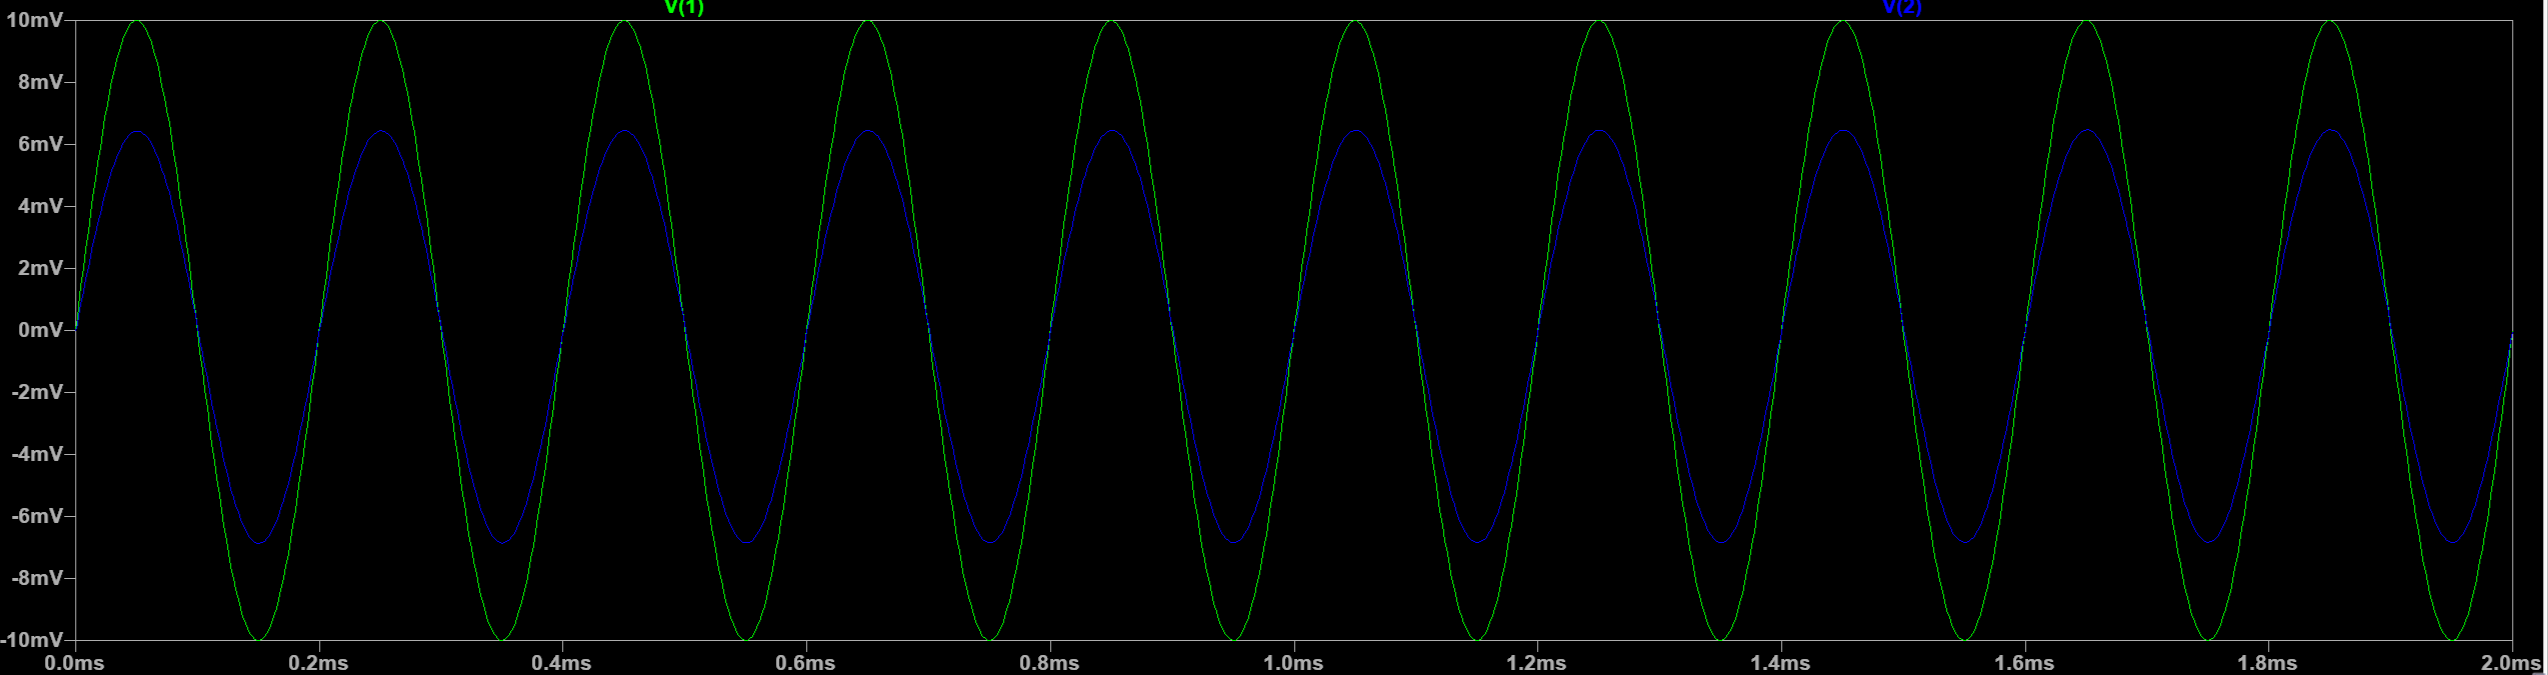
\includegraphics[width=\textwidth]{simulation/common_emitter_VsGreen_ViBlue.png}
        \caption{$v_s$ (Green) and $v_i$ (Blue)}
    \end{subfigure}
    \\[1em]
    \begin{subfigure}[b]{0.9\textwidth}
        \centering
        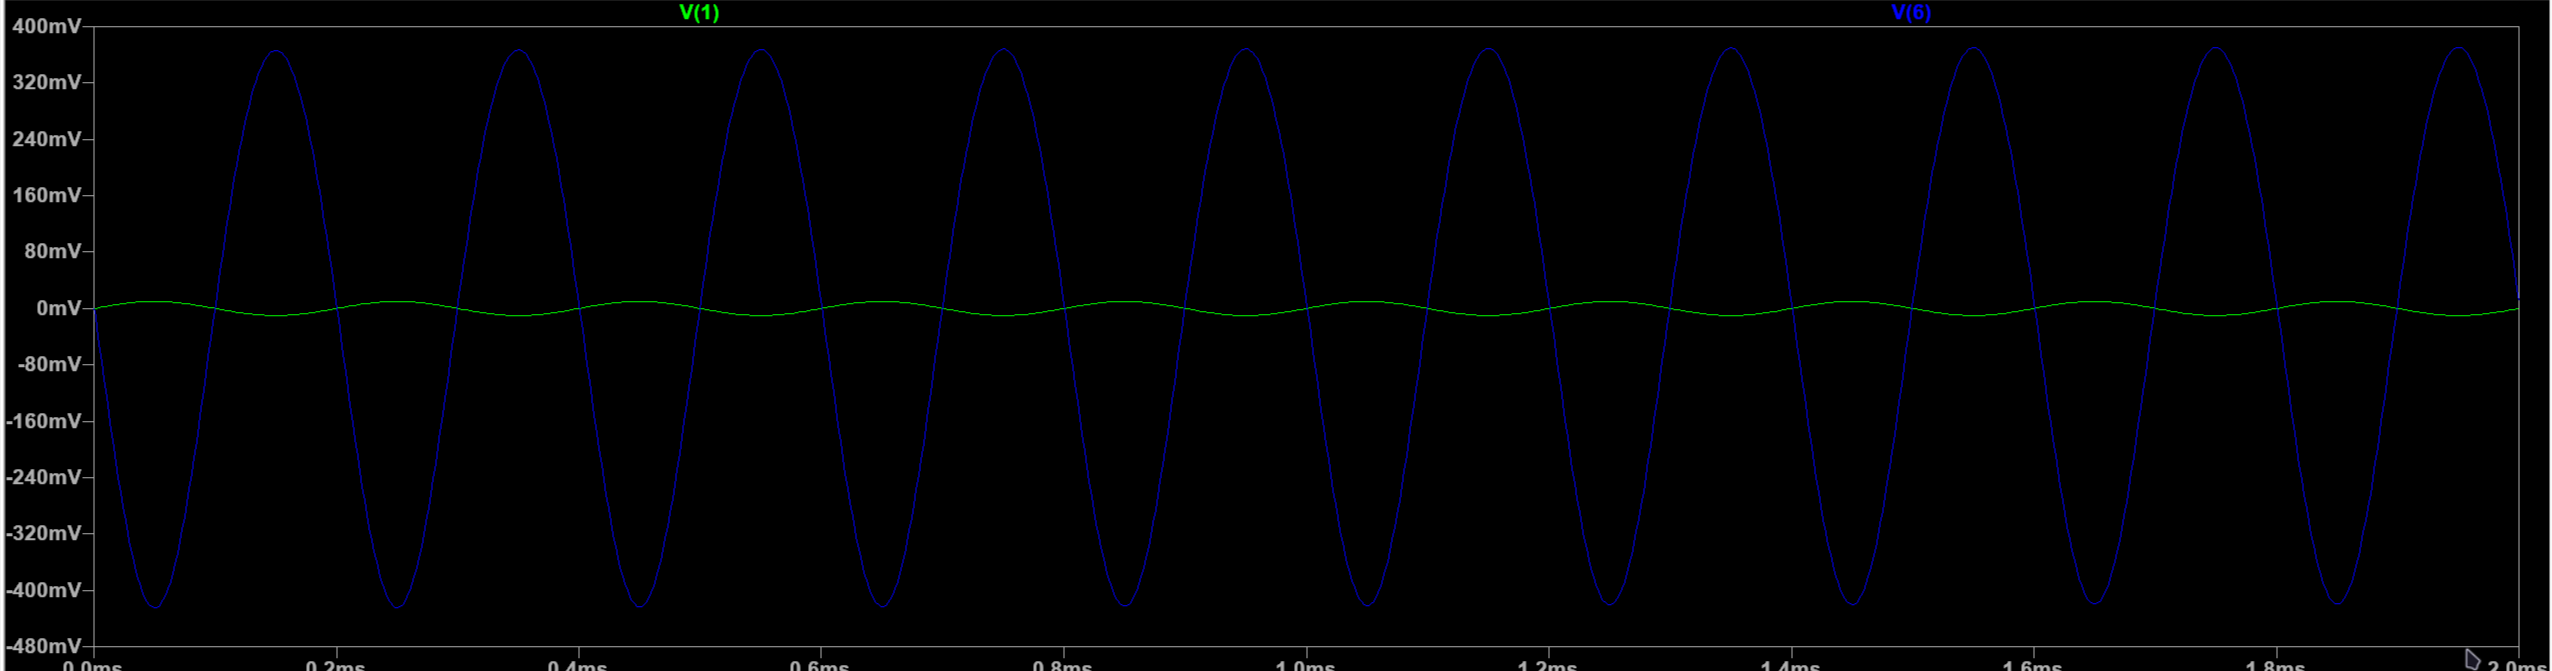
\includegraphics[width=\textwidth]{simulation/common_emitter_VsGreen_VoBlue.png}
        \caption{$v_s$ (Green) and $v_o$ (Blue)}
    \end{subfigure}
    \caption{Common Emitter simulation waveforms.}
    \label{fig:ce_sim}
\end{figure}

\pagebreak
\subsection{Emitter Follower Simulation}
The simulation for the emitter-follower configuration confirmed the near-unity voltage gain and lack of phase shift. Figure \ref{fig:ef_sim} shows the source voltage ($v_s$) compared to the input voltage ($v_i$) and the output voltage at the emitter ($v_o$).

\begin{figure}[H]
    \centering
    \begin{subfigure}[b]{0.9\textwidth}
        \centering
        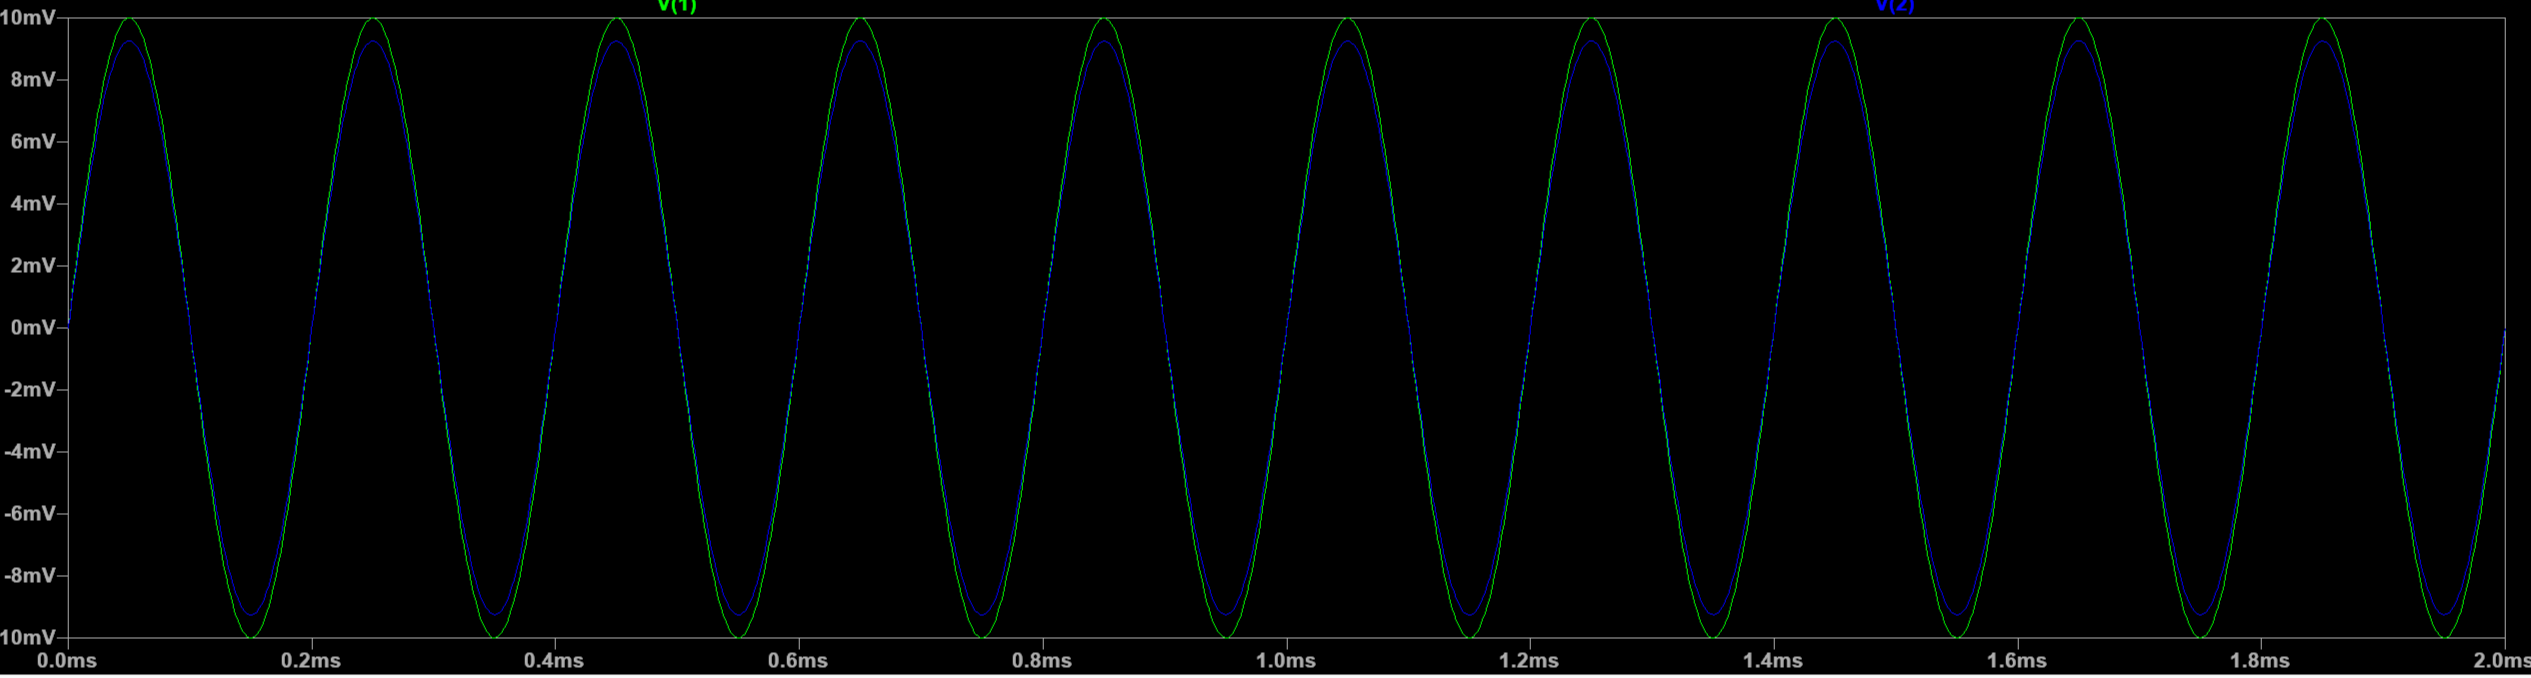
\includegraphics[width=\textwidth]{simulation/emitter_follower_VsGreen_ViBlue.png}
        \caption{$v_s$ (Green) and $v_i$ (Blue)}
    \end{subfigure}
    \\[1em]
    \begin{subfigure}[b]{0.9\textwidth}
        \centering
        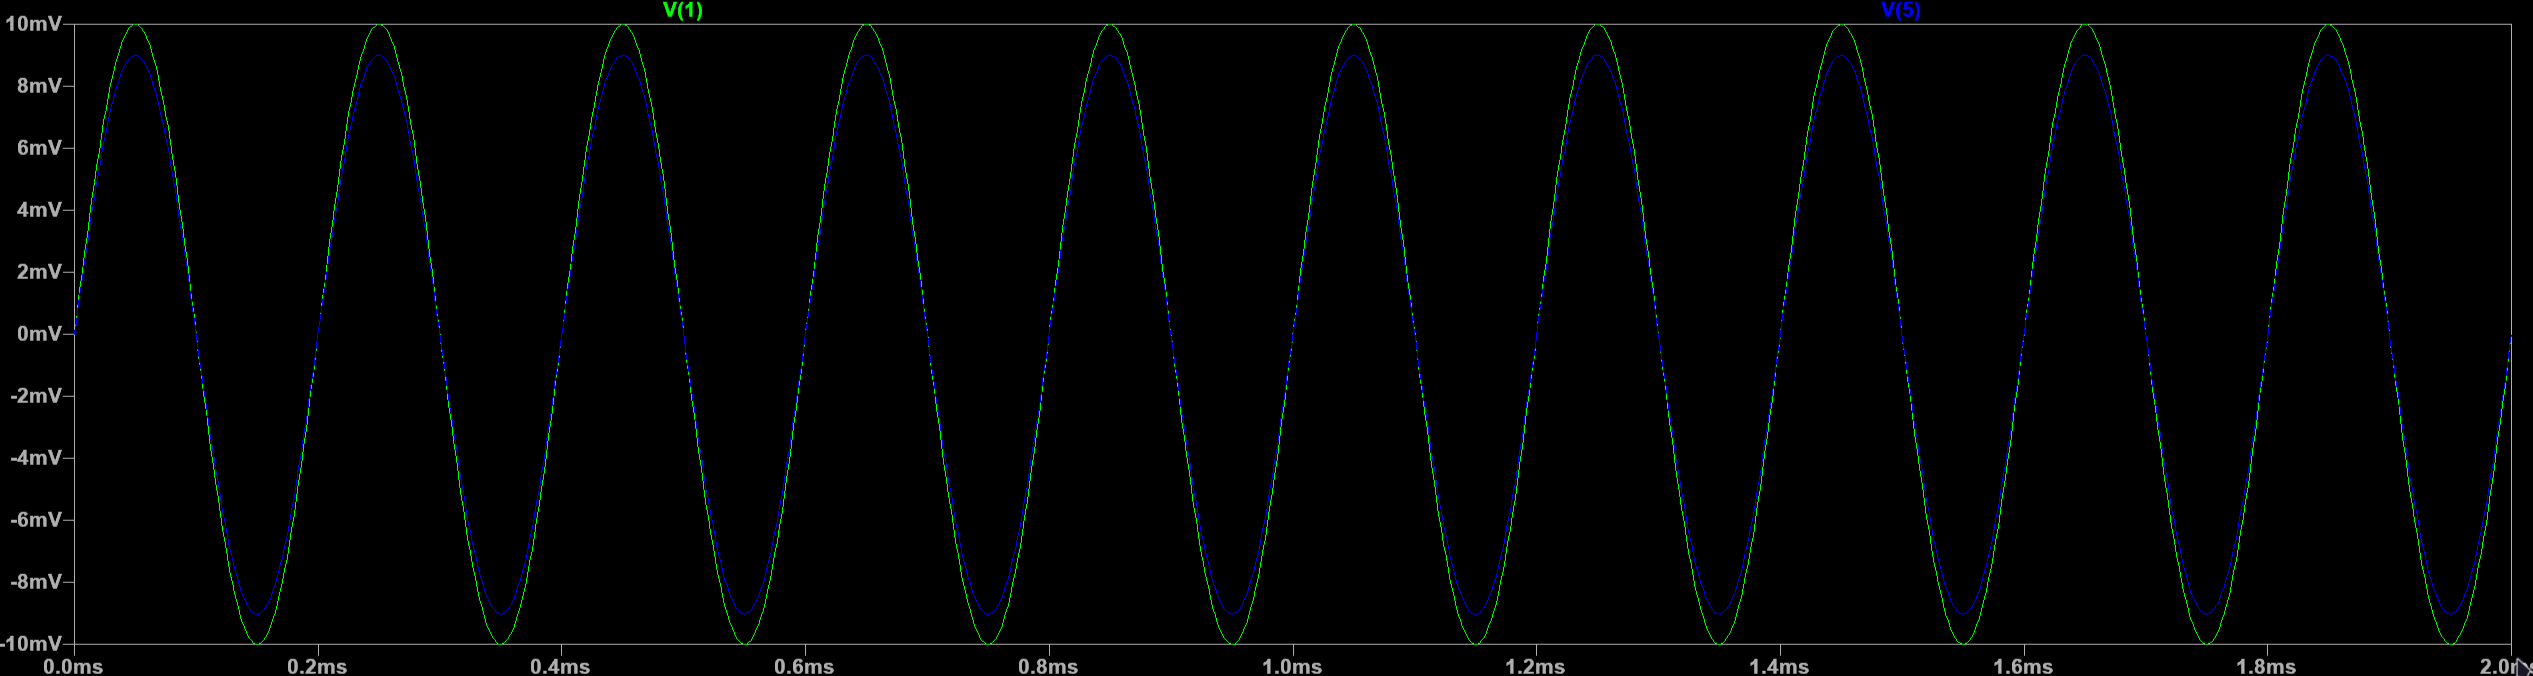
\includegraphics[width=\textwidth]{simulation/emitter_follower_VsGreen_VoBlue.png}
        \caption{$v_s$ (Green) and $v_o$ (Blue)}
    \end{subfigure}
    \caption{Emitter Follower simulation waveforms.}
    \label{fig:ef_sim}
\end{figure}

\pagebreak
%----------------------------------------------------------------------------------------
%	4. RESULTS AND DISCUSSION
%----------------------------------------------------------------------------------------
\section{Results and Discussion}

\subsection{Common Emitter Amplifier Performance}
The CE amplifier was assembled as shown in Figure \ref{fig:ce_bb}. The amplifier exhibited the expected phase inversion (180$^\circ$) and significant voltage gain.

\begin{figure}[H]
    \centering
    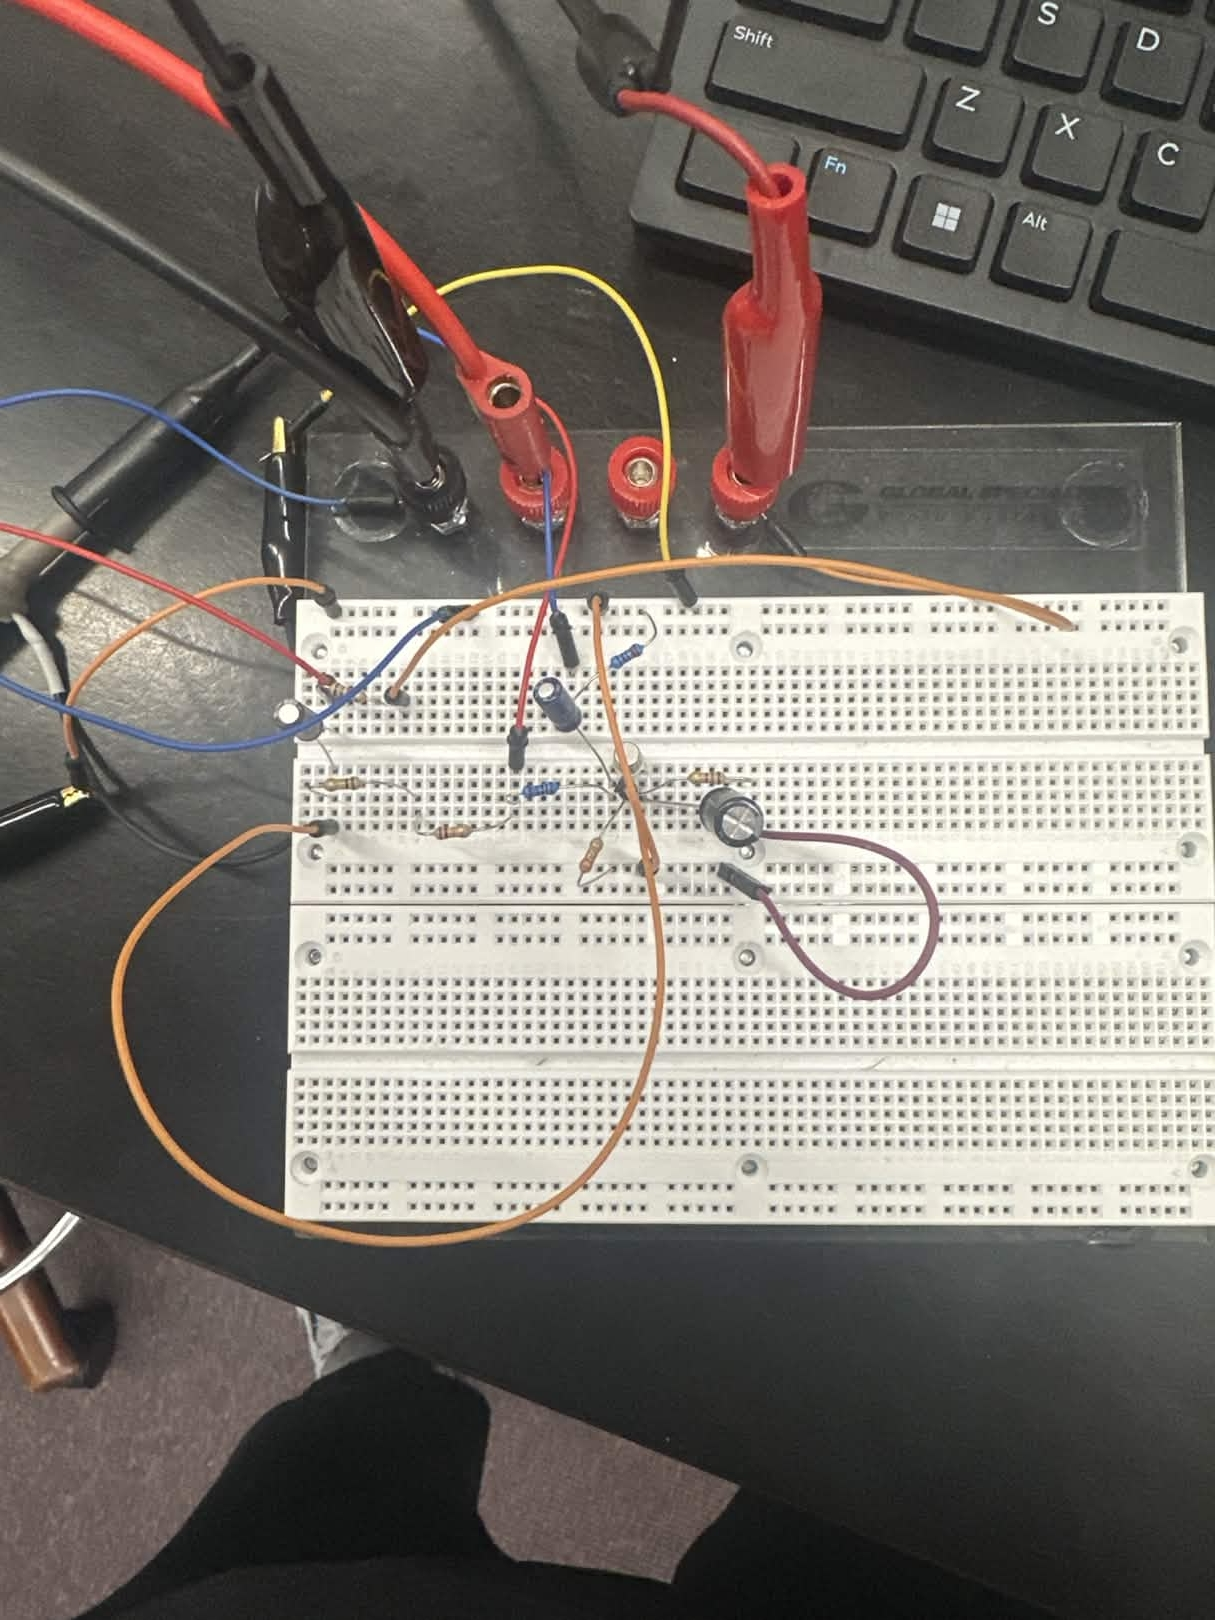
\includegraphics[width=0.5\textwidth]{common_emitter/breadboard.jpg}
    \caption{Breadboard assembly for the Common Emitter amplifier.}
    \label{fig:ce_bb}
\end{figure}

The measured waveforms for gain calculation are shown in Figure \ref{fig:ce_gain}. The green trace represents the input ($v_i$ or $v_s$) and the yellow trace represents the amplified output ($v_o$).

\begin{figure}[H]
    \centering
    \begin{subfigure}[b]{0.48\textwidth}
        \centering
        
\includegraphics[width=\textwidth]{common_emitter/part2_greenInputVi_yellowOutputVo.jpg}
        \caption{$v_i$ vs $v_o$}
    \end{subfigure}
    \hfill
    \begin{subfigure}[b]{0.48\textwidth}
        \centering
        
\includegraphics[width=\textwidth]{common_emitter/part2_greenInputVs_yellowOutputVo.jpg}
        \caption{$v_s$ vs $v_o$}
    \end{subfigure}
    \caption{CE amplifier input/output waveforms.}
    \label{fig:ce_gain}
\end{figure}

For $R_{in}$ and $R_{out}$ calculations, the peak voltages were recorded under various loading conditions (Figures \ref{fig:ce_res} and \ref{fig:ce_out_res}).

\begin{figure}[H]
    \centering
    \begin{subfigure}[b]{0.32\textwidth}
        \centering
        
\includegraphics[width=\textwidth]{common_emitter/part3_Vs.jpg}
        \caption{Measured $v_s$}
    \end{subfigure}
    \hfill
    \begin{subfigure}[b]{0.32\textwidth}
        \centering
        
\includegraphics[width=\textwidth]{common_emitter/part3_Vi.jpg}
        \caption{Measured $v_i$}
    \end{subfigure}
    \hfill
    \begin{subfigure}[b]{0.32\textwidth}
        \centering
        \includegraphics[width=\textwidth]{common_emitter/part3_Is.jpg}
        \caption{Voltage across $R_s$ ($i_s$)}
    \end{subfigure}
    \caption{CE measurements for input resistance calculation.}
    \label{fig:ce_res}
\end{figure}

\begin{figure}[H]
    \centering
    \begin{subfigure}[b]{0.48\textwidth}
        \centering
        
\includegraphics[width=\textwidth]{common_emitter/part4_RL_connected.jpg}
        \caption{$v_L$ (with $R_L$)}
    \end{subfigure}
    \hfill
    \begin{subfigure}[b]{0.48\textwidth}
        \centering
        
\includegraphics[width=\textwidth]{common_emitter/part4_RL_disconnected.jpg}
        \caption{$v_o$ (without $R_L$)}
    \end{subfigure}
    \caption{CE measurements for output resistance calculation.}
    \label{fig:ce_out_res}
\end{figure}

\pagebreak
\subsection{Emitter Follower Performance}
The Emitter Follower (Figure \ref{fig:ef_bb}) showed no phase inversion and a voltage gain slightly less than unity, as predicted by theory.

\begin{figure}[H]
    \centering
    
\includegraphics[width=0.5\textwidth]{emitter_follower/breadboard.jpg}
    \caption{Breadboard assembly for the Emitter Follower.}
    \label{fig:ef_bb}
\end{figure}

The waveforms in Figure \ref{fig:ef_gain} confirm that the output "follows" the input closely in both phase and amplitude.

\begin{figure}[H]
    \centering
    \begin{subfigure}[b]{0.48\textwidth}
        \centering
        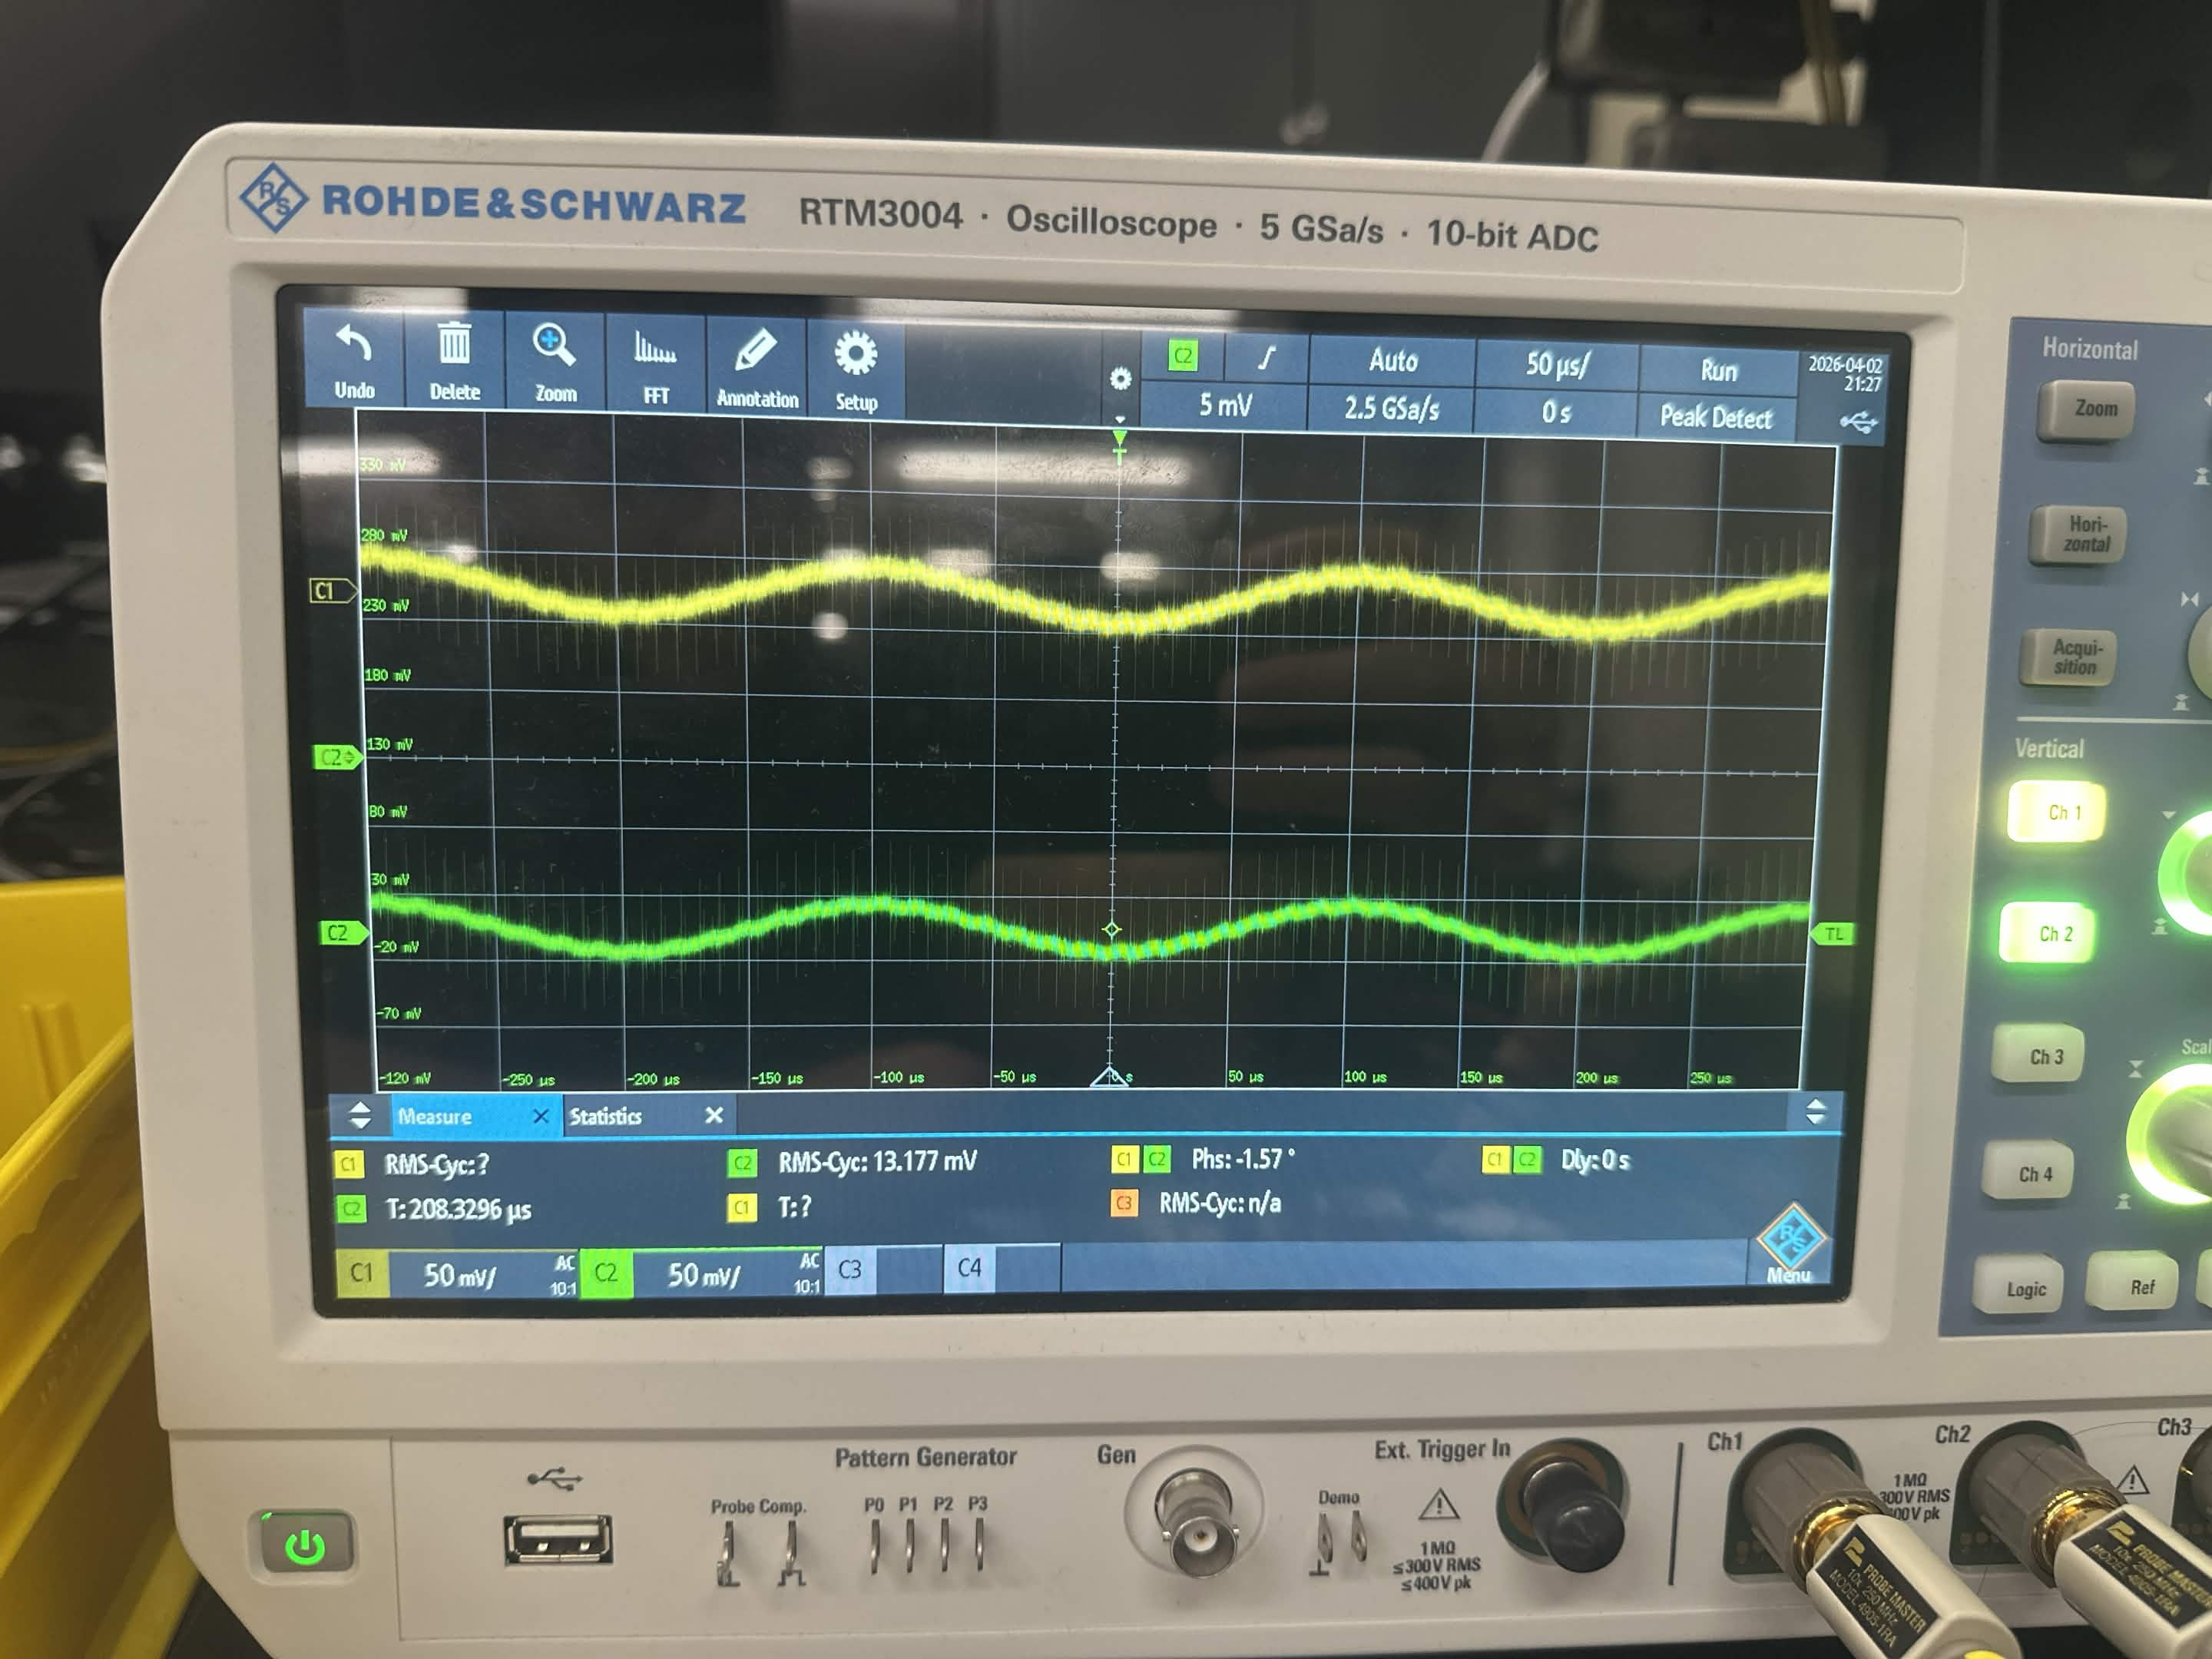
\includegraphics[width=\textwidth]{emitter_follower/part2_greenInputVi_yellowOutputVo.jpg}
        \caption{$v_i$ vs $v_o$}
    \end{subfigure}
    \hfill
    \begin{subfigure}[b]{0.48\textwidth}
        \centering
        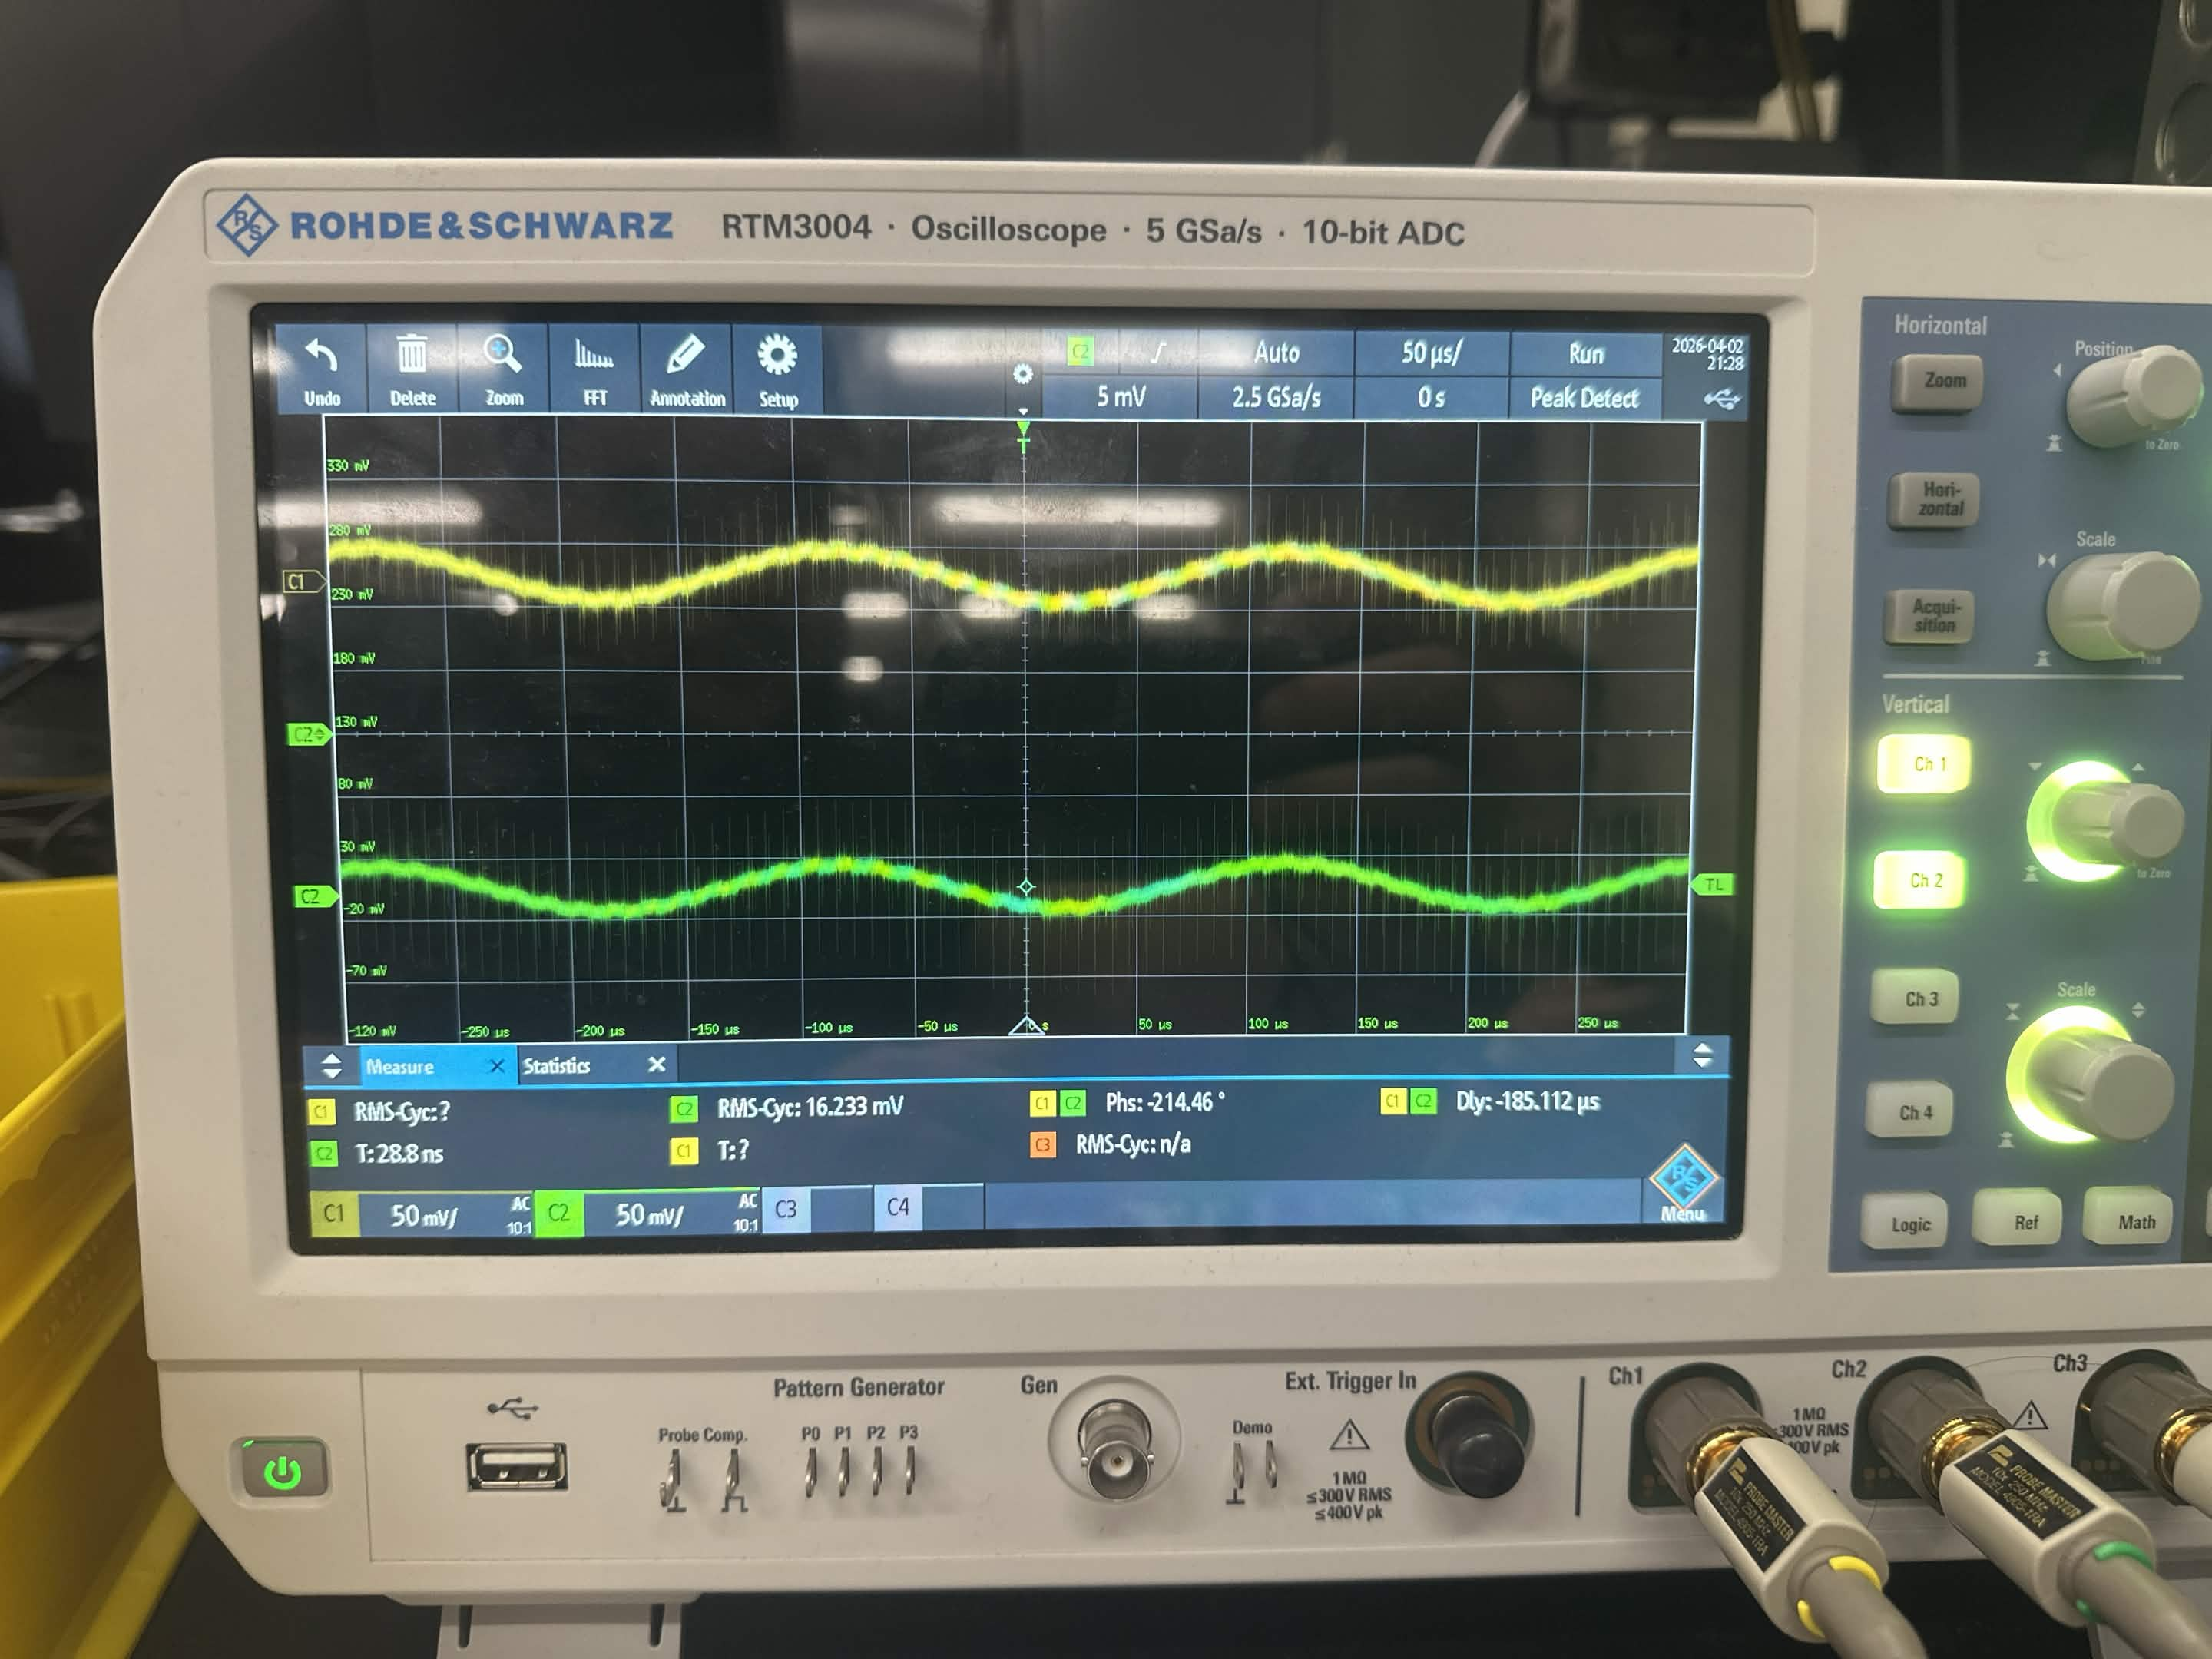
\includegraphics[width=\textwidth]{emitter_follower/part2_greenInputVs_yellowOutputVo.jpg}
        \caption{$v_s$ vs $v_o$}
    \end{subfigure}
    \caption{Emitter Follower input/output waveforms.}
    \label{fig:ef_gain}
\end{figure}

The input and output resistance measurements for the EF configuration are shown in Figures \ref{fig:ef_in_res} and \ref{fig:ef_out_res}. The EF showed significantly higher $R_{in}$ and lower $R_{out}$ compared to the CE amplifier.

\begin{figure}[H]
    \centering
    \begin{subfigure}[b]{0.48\textwidth}
        \centering
        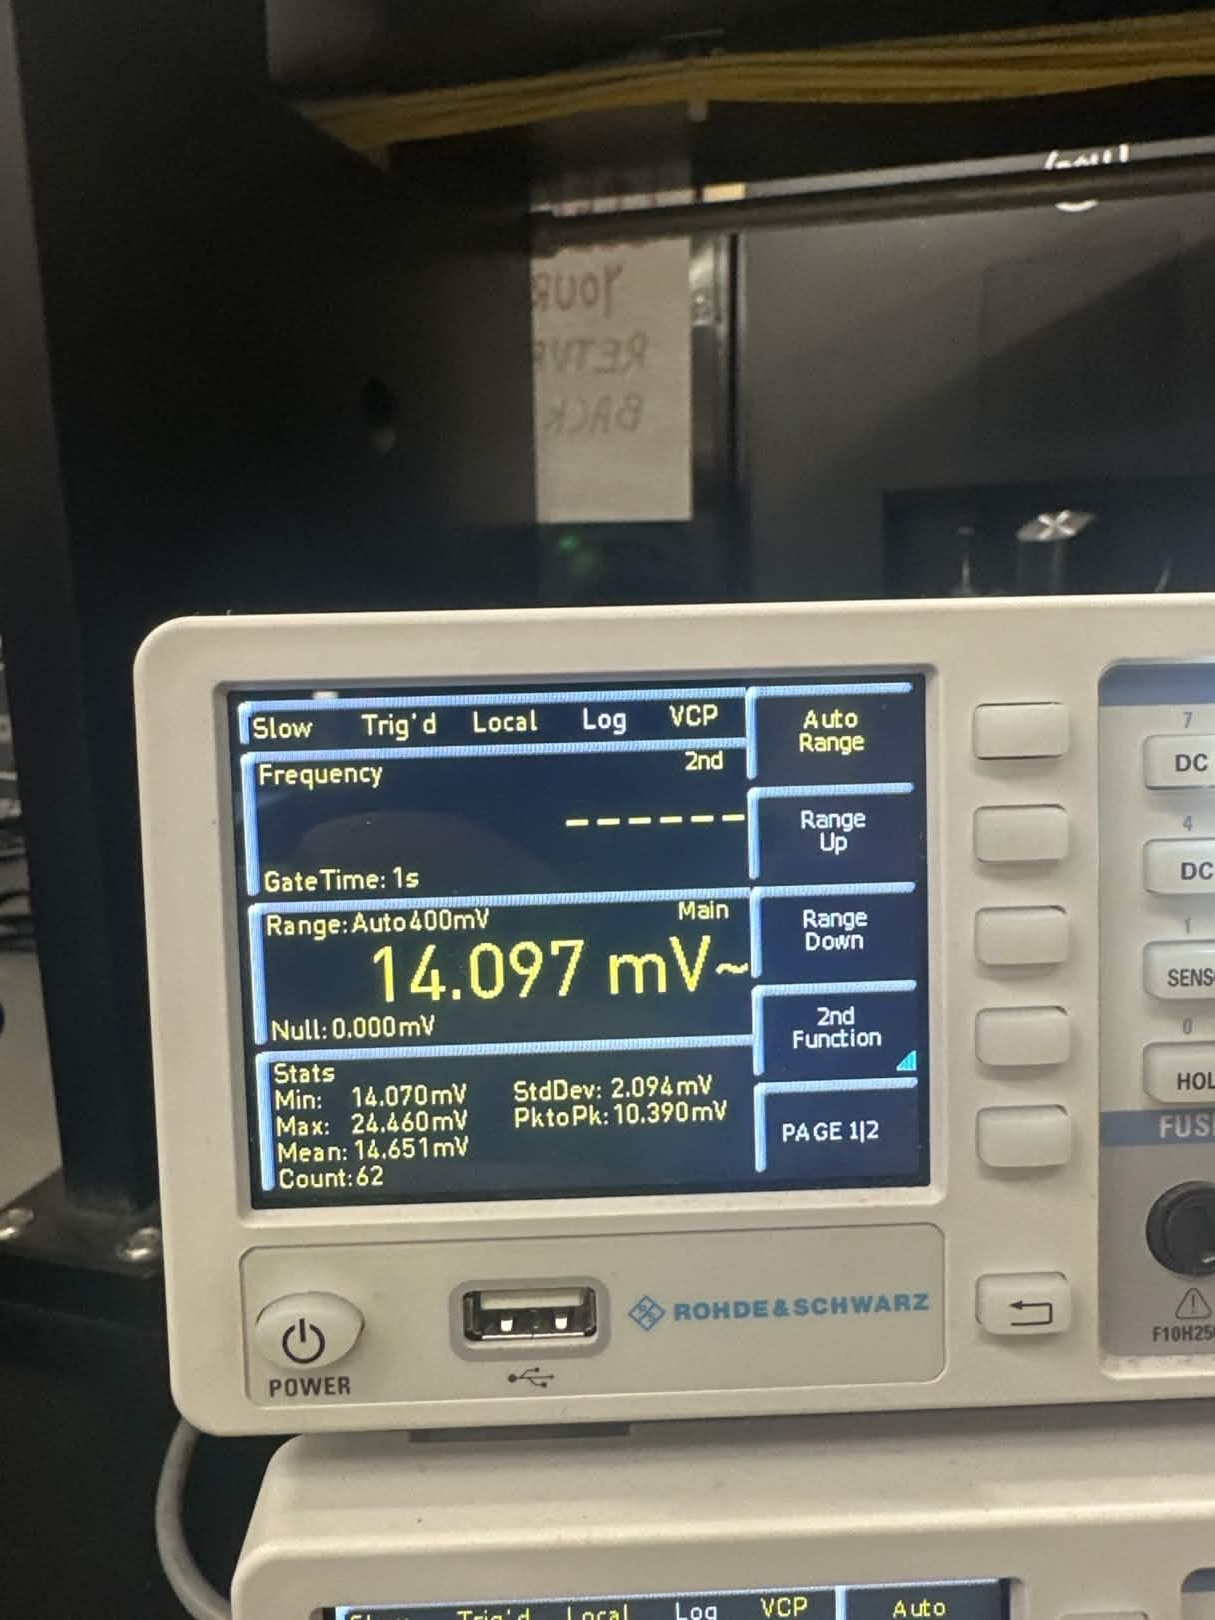
\includegraphics[width=\textwidth]{emitter_follower/part3_Vs.jpg}
        \caption{Measured $v_s$}
    \end{subfigure}
    \hfill
    \begin{subfigure}[b]{0.48\textwidth}
        \centering
        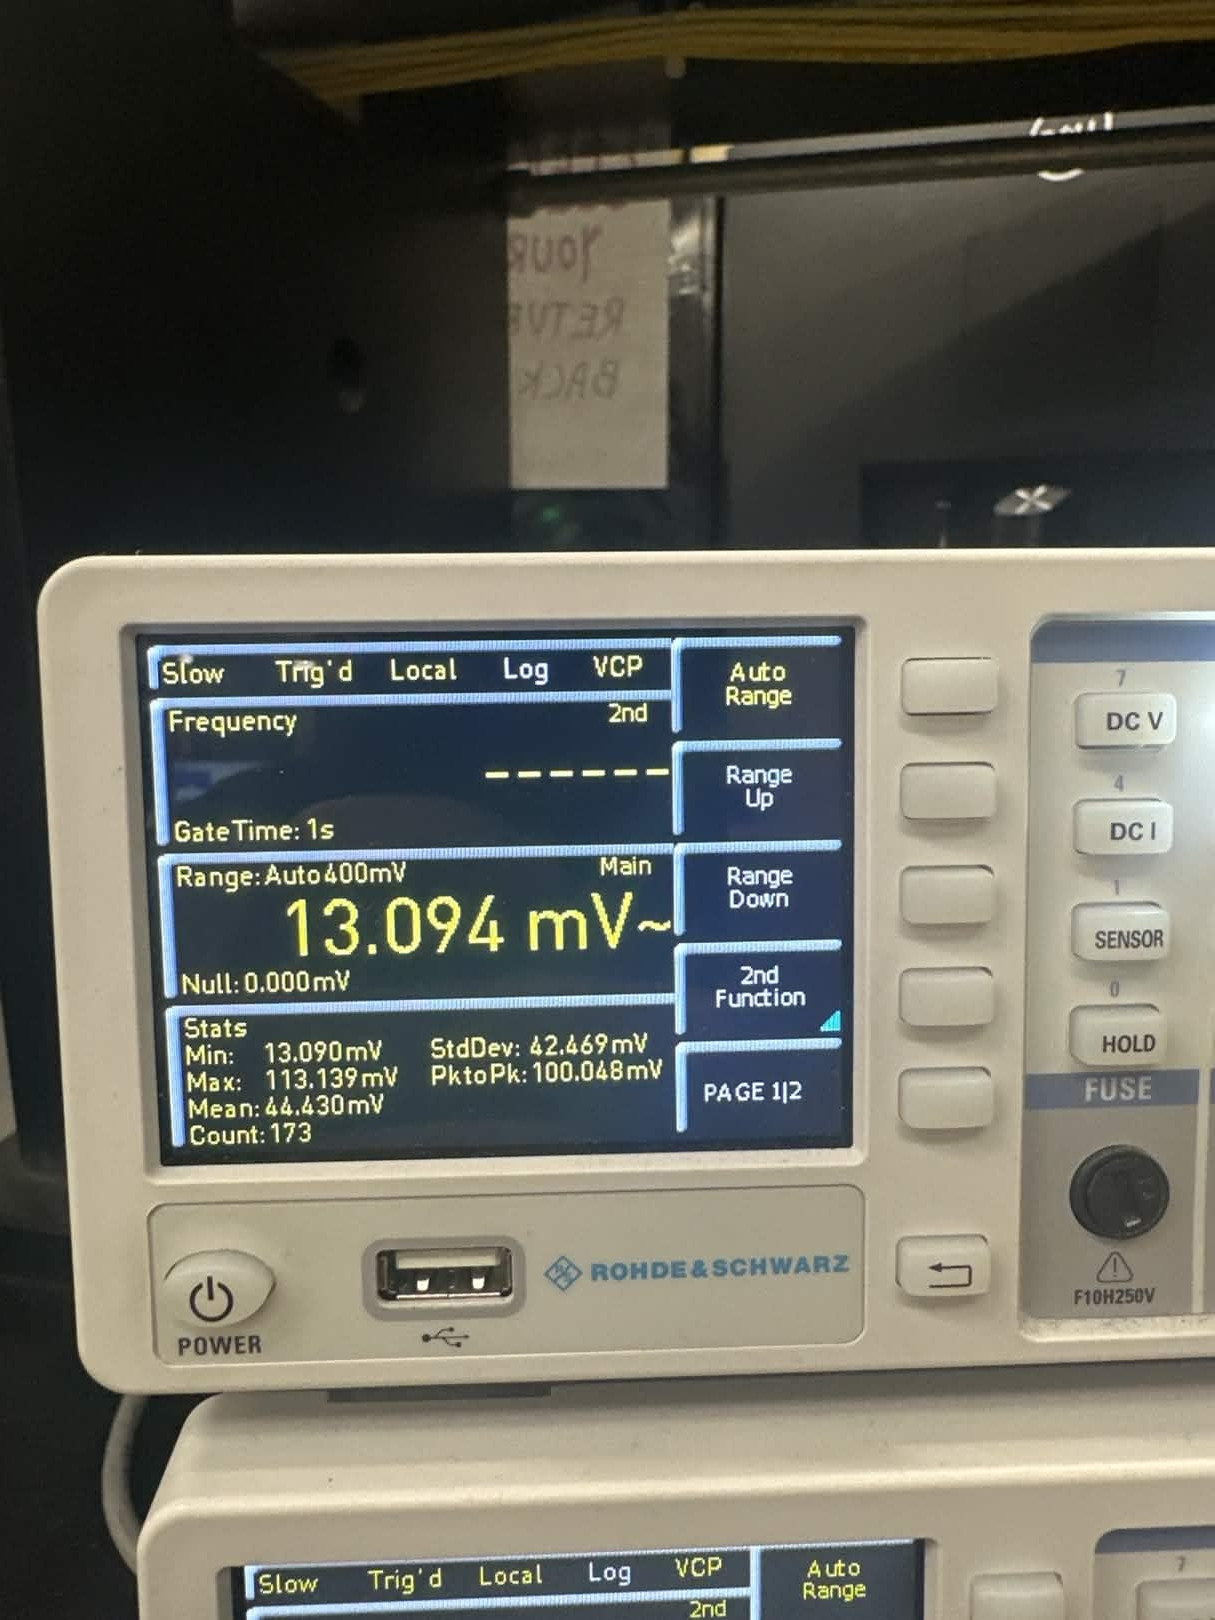
\includegraphics[width=\textwidth]{emitter_follower/part3_Vi.jpg}
        \caption{Measured $v_i$}
    \end{subfigure}
    \caption{EF measurements for input resistance calculation.}
    \label{fig:ef_in_res}
\end{figure}

\begin{figure}[H]
    \centering
    \begin{subfigure}[b]{0.48\textwidth}
        \centering
        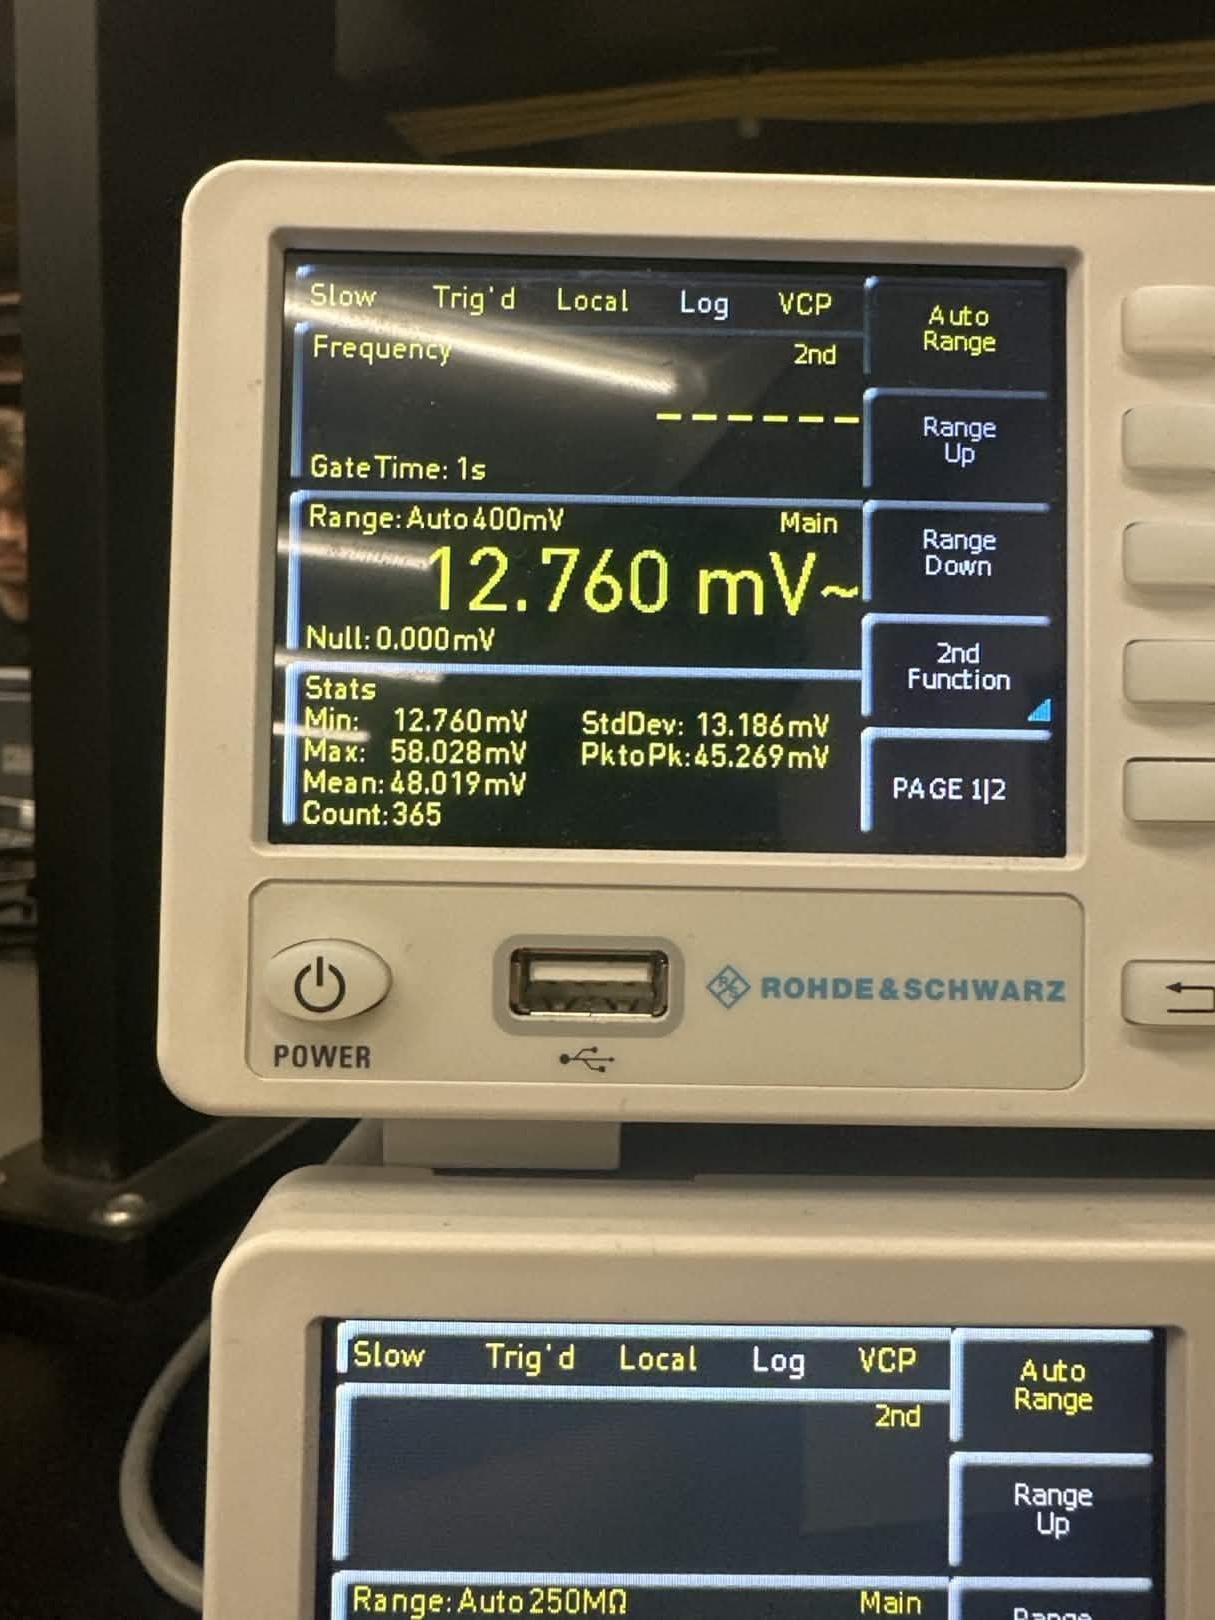
\includegraphics[width=\textwidth]{emitter_follower/part4_RL_connected.jpg}
        \caption{$v_L$ (with $R_L$)}
    \end{subfigure}
    \hfill
    \begin{subfigure}[b]{0.48\textwidth}
        \centering
        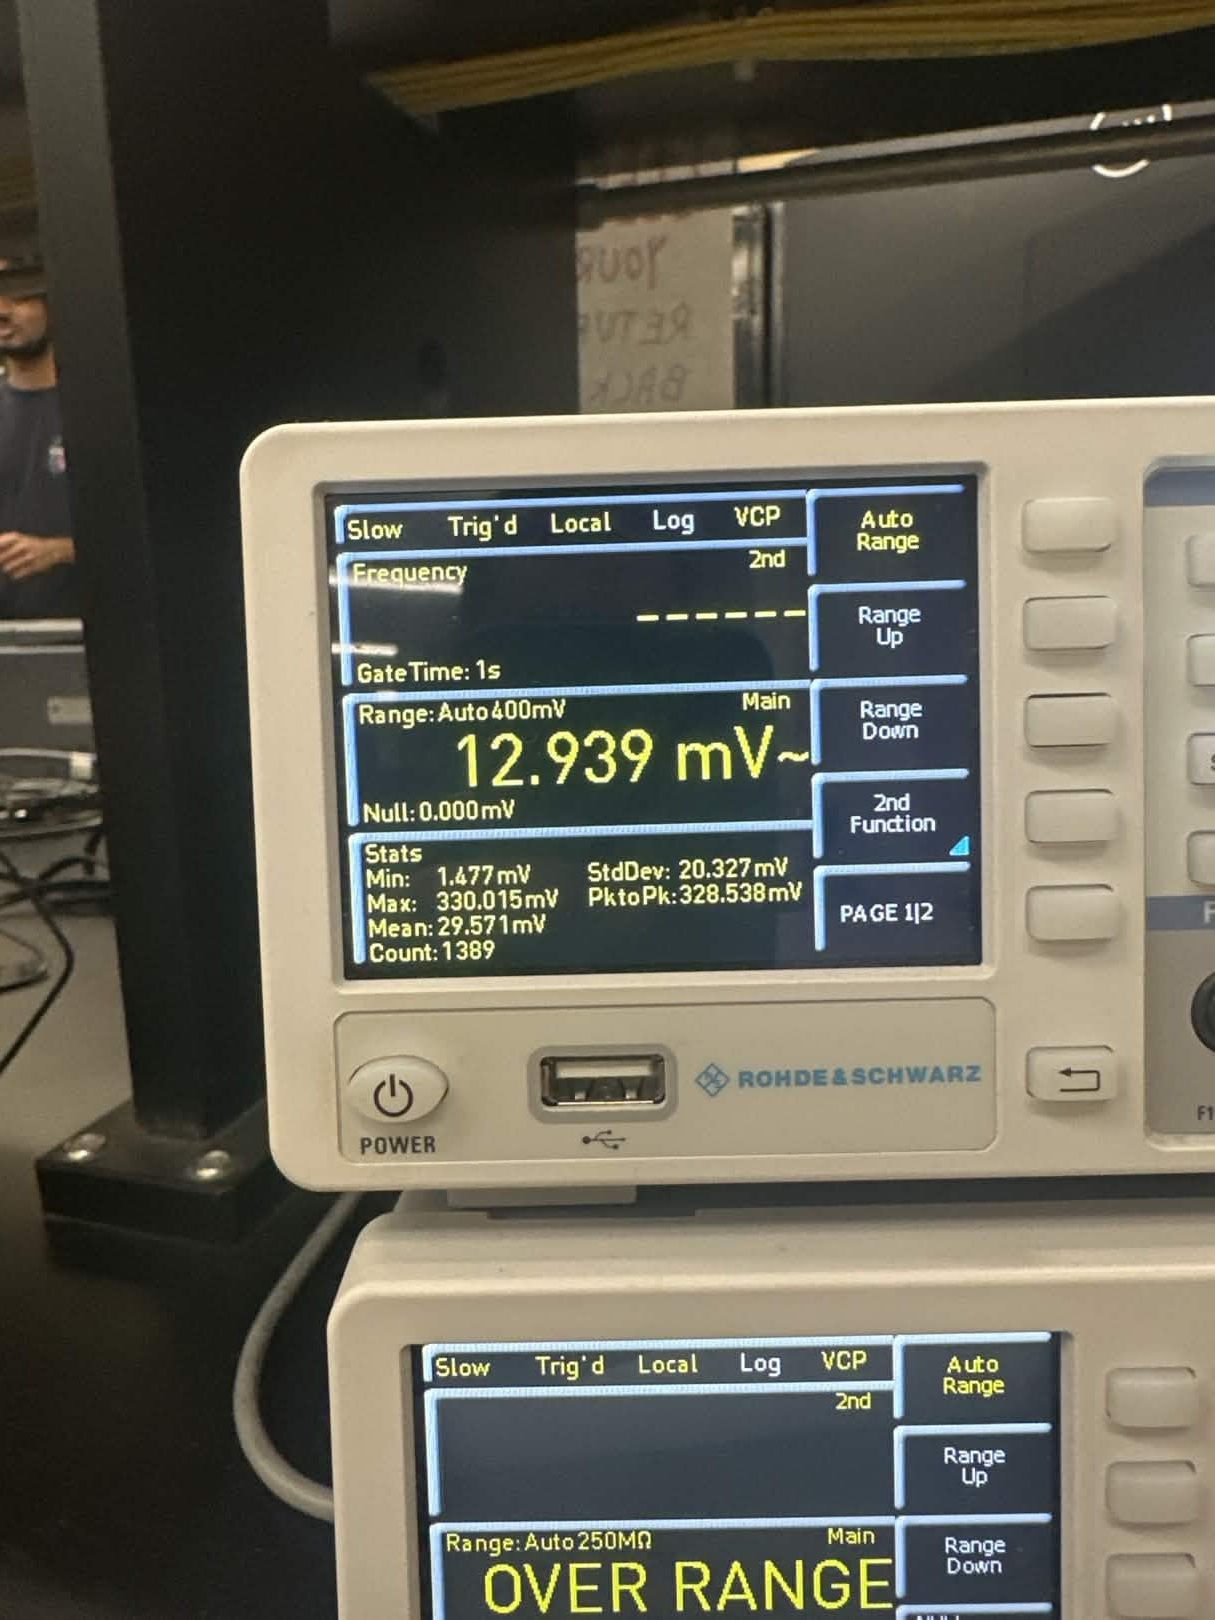
\includegraphics[width=\textwidth]{emitter_follower/part4_RL_disconnected.jpg}
        \caption{$v_o$ (without $R_L$)}
    \end{subfigure}
    \caption{EF measurements for output resistance calculation.}
    \label{fig:ef_out_res}
\end{figure}

\clearpage
%----------------------------------------------------------------------------------------
%	4. PRE-LABORATORY CALCULATIONS
%----------------------------------------------------------------------------------------
\section{Pre-Laboratory Calculations}
The theoretical derivations and calculations performed prior to the lab are attached below. These include the targeting of $I_{CQ} = 1mA$ and the derivation of the small-signal models for both CE and EF configurations.
\pagebreak
\includepdf[pages=-]{prelab.pdf}

%----------------------------------------------------------------------------------------
%	5. CONCLUSION
%----------------------------------------------------------------------------------------
\section{Conclusion}
The experiment successfully demonstrated the characteristics of common-emitter and emitter-follower amplifiers. The CE configuration provided high voltage gain (measured $Av_i \approx -62$) and phase inversion, making it suitable for signal amplification. However, its relatively low input resistance and high output resistance ($R_{out} \approx R_C$) limit its effectiveness in impedance matching. Conversely, the Emitter Follower provided a gain near unity ($\approx 0.97$) with no phase shift, but excelled in providing high input resistance and very low output resistance. This confirms the EF's primary application as a buffer stage for impedance matching between high-impedance sources and low-impedance loads.
\end{document}
